% +--------------------------------------------------------------------+
% | Sample Chapter 3
% +--------------------------------------------------------------------+

\cleardoublepage

% +--------------------------------------------------------------------+
% | Replace "This is Chapter 3" below with the title of your chapter.
% | LaTeX will automatically number the chapters.
% +--------------------------------------------------------------------+

\chapter{Exploración Hardware}
\label{makereference3}

El primer hito a nivel técnico era encontrar una placa de desarrollo que incluyera Bluetooth de bajo consumo y permitiera conectar un sensor de acelerometría, ya que eran indispensables para la transmisión de datos entre la placa y el dispositivo móvil. 

Desde el punto de vista comercial, la intención ha sido buscar el componente con mejores prestaciones en calidad y precio con el objetivo de preparar un producto final que pudiera competir con otras opciones del mercado.

Destacamos las placas con Bluetooth incorporado y un microprocesador. En la tabla~\ref{tablaSoCBLE} observamos el análisis de cada elemento que se ha considerado.

\begin{table} % TODO marcar en un color las opciones elegidas
	\begin{center}
	\begin{tiny}
	\begin{tabular}[c]{|c|c|c|c|c|c|}
        \hline
        \multicolumn{6}{|c|}{CHIPS CON BLUETOOTH} \\
        \hline
        EMPRESA & MODELO & PROCESADOR & FLASH & RAM & I/O \\
        \hline
        Nordic & PTR9022 & ARM Cortex-M0 & 256 KB & 16 KB & SPI, 2-WIRE, UART \\
		\rowcolor{Green}Nordic & nRF51-DK & ARM Cortex-M0 & 256/128KB & 32KB/16KB & SPI Master/Slave, 2-wire, UART, 31 GPIO \\
		Nordic & nRF51422 & ARM Cortex-M0 & 256/128KB & 16KB & SPI Master/Slave, 2-wire, UART, 31 GPIO \\
		TI & CC2540 / CC2541 & 8051 & 128/256KB & 8KB & 2 USART, ADC, 21 GPIO, SPI \\
		TI & CC2640F128RGZT & ARM Cortex-M3 & 128KB & 20KB & I2C, I2S, SPI, UART \\
		\rowcolor{Green}Cypress & 4 BLE/PRoC BLE & ARM Cortex-M0 & 128/256KB & 16/32KB & 2 SCBs, configurable como I2C, SPI o UART \\
		Cypress & PSoC 4XX7-BLE & ARM Cortex-M0 & 128KB & 16KB & I2C, SPI, UART, 36 GPIO \\
    	\hline
	\end{tabular}
	\end{tiny}
    \caption{Placas que integran radio Bluetooth Low Energy. Se destacan las alternativas seleccionadas para la siguiente fase de exploración}
    \label{tablaSoCBLE}
   \end{center}
\end{table}

Dada la naturaleza de nuestro proyecto no necesitábamos un gran poder de procesamiento ni una gran capacidad en cuanto a memoria RAM y flash, ya que el código iba a ser muy sencillo. Los dos factores principales a tener en cuenta eran que incorporase la tecnología Bluetooth Low Energy y que permitiese la conexión y el envío de datos con el acelerómetro, ya fuera mediante I2C, SPI, UART...

Realizando el primer filtro pudimos observar que algunas características eran comunes entre los SoC’s elegidos:

En materia de procesadores encontramos dos opciones comunes: \textbf{Cortex-M0} de ARM (Advanced RISC Machines) y \textbf{8051} de Intel. Al ver que la mayoría de los chip elegidos montaban el procesador de ARM, claramente observamos que domina el mercado de los sistemas empotrados y las empresas han optado por utilizarlo. Esto se debe a que el modelo de negocio utilizado por ARM consiste en la venta de licencias de sus núcleos~\cite{ARMIPCore}, lo que permite a otros fabricantes diseñar su propio System On Chip (SoC) integrando tecnología ARM.

ARM Cortex-M0 nos parecía una opción más interesante, ya que este procesador tipo RISC, cuenta tanto con una arquitectura de 32 bits (frente a los 16 de Intel 8051) como con la arquitectura \textit{Thumb}, que mejora la densidad del código para ocupar menos espacio tanto en memoria RAM como en flash.

La cantidad de memoria RAM disponible más común para este tipo de dispositivos es de 8, 16 o 32 kilobytes. La segunda opción nos pareció más que suficiente para albergar un programa sencillo como el nuestro y las variables necesarias.

En cuanto a capacidad de almacenamiento, todas las placas cuentan con memoria flash, que pueden variar entre 128 y 256 Kilobytes. De nuevo, la complejidad de nuestro programa no iba a generar un fichero compilado de gran tamaño, y no necesitábamos guardar nada más, por lo que 128 KB nos parecieron adecuados.

En cuanto a los periféricos de entrada/salida, la mayoría de las placas de desarrollo incluyen los protocolos SPI e I2C.

El protocolo SPI consiste en el envío de la señal de reloj del maestro y en cada impulso de reloj se envía un bit al esclavo y recibe un bit de éste. Los nombres de las señales son SCK para el reloj, MOSI para el Maestro Out Esclavo In, y MISO para Maestro In Esclavo Out.

El protocolo I2C, usa dos cables, uno para el reloj (SCL) y otro para el dato (SDA). El maestro y esclavo envían datos por el mismo cable, el cual es controlado por el maestro, que crea la señal de reloj. Este protocolo utiliza direccionamiento, es decir, el primer byte enviado por el maestro se forma de 7 bits para la dirección (así que permite comunicarse con hasta 127 dispositivos) y un bit de lectura/escritura, indicando si el próximo byte vendrá desde el maestro o el esclavo. Esta tecnología se ampliará en el Capítulo~\ref{makereference5.1.1}.

\section{Selección de plataformas de desarrollo}
\label{makereference3.3}

Una vez recopilados los modelos de que observamos en la Tabla~\ref{tablaSoCBLE}, hemos destacado 2 placas de prototipado que cumplen con los requisitos del proyecto. Este tipo de placas ofrecen más características de las que necesitamos para el proyecto, pero suponen un primer paso para poder programar y realizar pruebas antes de pasar a chips más simples y con un menor coste. 

Por un lado escogimos la placa de desarrollo de Cypress con el kit PSoC BLE y modelo de la placa con Bluetooth \textbf{CY8CKIT-042-BLE} certificado para sistemas de bajo consumo. Es un kit provisto de un chip que ofrece un procesador ARM Cortex-M0 y capacidad y conectividad suficiente como para utilizarlo de base para el proyecto.

El entorno de desarrollo para las plataformas de Cypress es un software de escritorio llamado \textit{PSoC Creator}, en el cual podemos diseñar sistemas a través de un panel gráfico. Nos ofrece multitud de librerías disponibles para la placa utilizada y es posible codificar, compilar, y depurar código.\\

Consideramos también la placa de Nordic modelo \textbf{nRF51-DK} por ser un kit de desarrollo que ofrece el mismo procesador que Cypress, conectividad tanto I2C como SPI para realizar las pruebas con el sensor. 
Este modelo ofrece compatibilidad con la plataforma de desarrollo \textit{mbed} de ARM, es una opción que nos resultó interesante a la hora escogerla. Dispone de una gran comunidad y soporte lo cual es de agradecer.\\

En la Sección~\ref{makereference3.4} hablaremos más sobre los aspectos específicos de ambos entornos de desarrollo.

Al considerar que era más interesante tener una placa con procesador, sensores y periféricos descartamos los chips individuales y optamos por una opción más completa.

\subsection{Análisis de las plataformas escogidas}
\label{makereference3.4}

Rápidamente observamos dos grandes empresas especializadas en el sector como son Nordic y Cypress. Tienen gran variedad de microprocesadores y placas de desarrollo que cumplen con nuestras expectativas.

Elegimos el kit de desarrollo de Nordic (\textbf{nRF51-DK}), que incluye Bluetooth Smart e incorpora un núcleo ARM Cortex-M0 32-bit como la mayoría de los chips que encontramos. Una memoria flash a 256/128KB con RAM de 32KB/16KB para mejorar el rendimiento de las aplicaciones.

El kit permite el acceso a todas las interfaces de entrada y salida como SPI Master/Slave, 2-wire, UART y 31 GPIOs a través de conectores. Tiene 4 LED’s y ofrece también 4 botones que son programables por el usuario. 

Utiliza un cable micro USB 2.0 para conectarse a uno de los puertos USB de el PC. Esto proporciona alimentación a la placa, y es compatible con la programación de destino.

\begin{figure}[h]%t=top, b=bottom, h=here
	\centering
    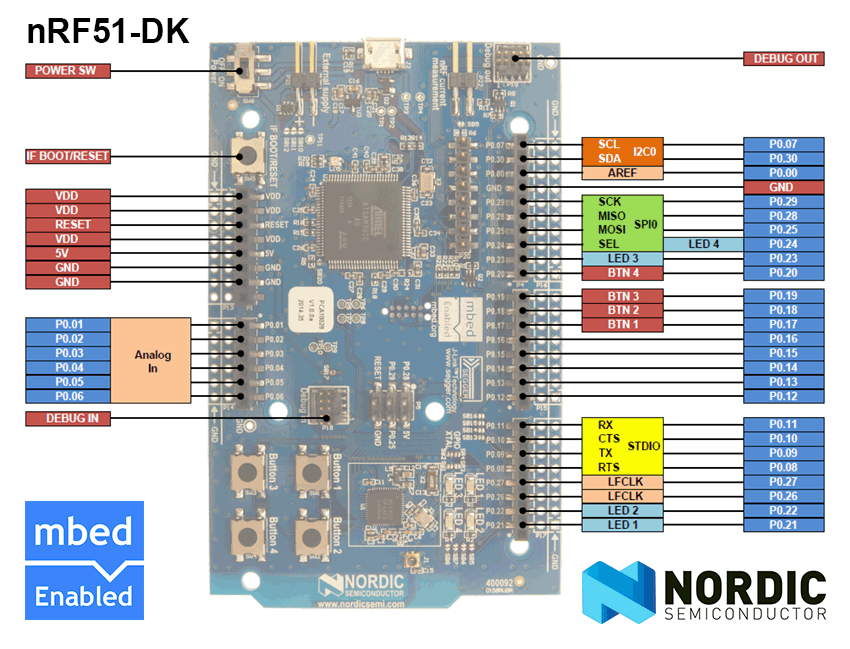
\includegraphics[scale=0.5]{figures/nRF51DK_pines.png} % TODO hacer que esto no quede horrible

    \caption[Esquema de la disposición de pines de la placa nRF51-DK de Nordic]{Esquema de la disposición de pines de la placa nRF51-DK de Nordic}

   \label{figuraNordicNRF51}
\end{figure}

La carga de programas resulta sencilla, ya que una vez conectado al ordenador, el sistema de archivos se monta como una unidad extraíble, por lo que solo debemos abrir un explorador de archivos y podremos cargar los programas a la placa arrastrando y soltando hacia la unidad.

%FIXME ESTO SIGUE PARECIENDO COPIADO
La placa de desarrollo nRF51-DK es compatible con el entorno \textbf{ARM mbed}, que es una plataforma gratuita de prototipado rápido y experimentación con microcontroladores ARM. Provee a los desarrolladores una plataforma para realizar pruebas y prototipos en el lenguaje de programación C++. Incluye una amplia variedad de librerías, tutoriales y ejemplos, además de contar de una gran comunidad online de desarrolladores de software, cuyos códigos son habitualmente accesibles a toda la comunidad.

Otro chip con procesador que nos pareció interesante fue el modelo \textbf{CY8CKIT-042-BLE} de la empresa Cypress Semiconductor que soporta 2 dispositivos: PSoC 4 BLE y PRoC BLE.

El modelo escogido es el PSoC 4 BLE que provee de una completa solución para conectividad Bluetooth Low Energy. También monta una procesador ARM Cortex-M0 con una memoria flash de 128kB/ 256kB y RAM de 16kB / 32kB. Dispone de 4 TCPWM1, 2 SCBs2, LCD4, I2S5, y 36 GPIOs.

\begin{figure}[h]%t=top, b=bottom, h=here
	\centering
    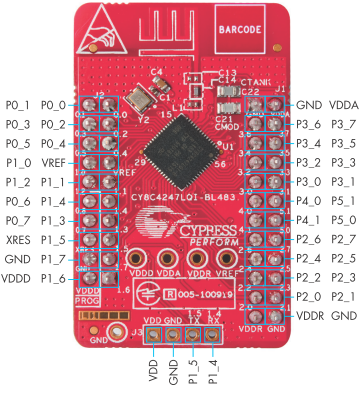
\includegraphics[scale=0.6]{figures/cypress_psoc.PNG} % TODO hacer que esto no quede horrible

    \caption[Cypress PSoC]{Cypress PSoC. Esta placa contiene el microchip y todos los conectores necesarios como para usarla directamente como producto final}

   \label{figuraCypressPeque}
\end{figure}

\begin{figure}[h]%t=top, b=bottom, h=here
	\centering
    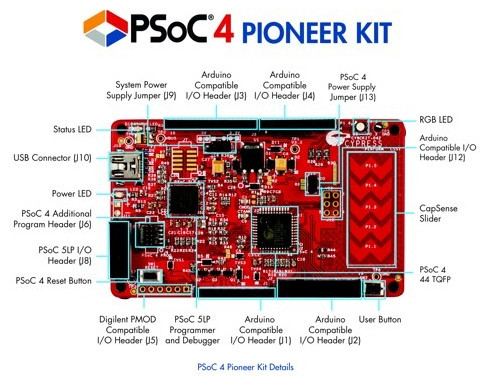
\includegraphics[scale=0.8]{figures/cypress_placa_desarrollo} % TODO hacer que esto no quede horrible

    \caption[PSoC 4 BLE, placa de desarrollo]{PSoC 4 BLE, placa de desarrollo, en esta placa se conecta el PSoC para poder programarlo, y añade más funcionalidad incorporando elementos como botones programables, un LED RGB, un panel deslizante, etc.}

   \label{figuraCypressGrande}
\end{figure}

El kit incluye una memoria extraible que conecta la placa por Bluetooth llamado Dongle USB CySmart (BLE Dongle) que se empareja con la herramienta de emulación principal CySmart. El emparejamiento con un entorno Windows hace que sea un potente entorno de depuración de Bluetooth LE.

Este kit de desarrollo de Cypress es compatible con diseños a nivel de sistema mediante PSoC Creator, un software de desarrollo que contiene numerosos proyectos de ejemplo para proporcionar diseños integrados de señal mixta Bluetooth de baja energía, el lenguaje utilizado es C.

Es sencilla diseñar pues con arrastrar y soltar los componentes se añaden al panel principal obteniendo máxima flexibilidad de diseño.

\section{Conclusión}
\label{makereference3.5}

Tanto la placa nRF51-DK de Nordic como CY8CKIT-042-BLE de Cypress son dos placas de desarrollo perfectas para iniciar un proyecto con conectividad Bluetooth, las dos tienen idénticas características, conectores y periféricos, se les puede incluir una pila de botón CR2032 para darles autonomía y les respalda un software para desarrollo de las mismas.

En este punto tuvimos cierta controversia, ya que el software de Mbed de Nordic nos da la posibilidad de compilar código C++ en cualquier PC con internet gracias a su versión web. Nos ofrece una gran comunidad que es de agradecer y mucho contenido de ejemplos y tutoriales en la web oficial. Por contra no tiene modo depuración por pasos y eso dificulta su seguimiento y depuración. 

Por otro lado, PSoC Creator de Cypress nos ofrece un completo programa de escritorio muy visual al diseñar circuitos y un sistema “drag and drop” muy intuitivo. Permite modo depuración facilitando su programación. Por contra nos hemos encontrado con ciertas dudas que han sido difíciles de resolver en foros debido al poco contenido sobre el tema.

Debido al gran parecido entre las características de una placa y otra, y a que los entornos de desarrollo tienen cada uno sus pros y sus contras, nos resultó difícil elegir una de las dos para finalizar el proyecto. En el Capítulo~\ref{makereference4} se hablará de las pruebas que realizamos con ambas y qué nos motivó a escoger la placa de Nordic frente a la de Cypress.